\documentclass[a4paper, 11pt]{article}
\usepackage[utf8]{inputenc}
\usepackage{amsmath}
\usepackage{array}
\usepackage{listings}
\usepackage{color}
\usepackage{caption}
\usepackage{varioref}
\usepackage[section]{placeins}
\usepackage{comment} % enables the use of multi-line comments (\ifx \fi) 
\usepackage{graphicx}
\usepackage{lipsum} %This package just generates Lorem Ipsum filler text. 
\usepackage{fullpage} % changes the margin
\usepackage{cleveref}
\definecolor{dkgreen}{rgb}{0,0.6,0}
\definecolor{gray}{rgb}{0.5,0.5,0.5}
\definecolor{mauve}{rgb}{0.58,0,0.82}

\DeclareMathOperator*{\argmax}{argmax} % thin space, limits underneath in displays

\newenvironment{conditions}
{\par\vspace{\abovedisplayskip}\noindent\begin{tabular}{>{$}l<{$} @{${}={}$} l}}
	{\end{tabular}\par\vspace{\belowdisplayskip}}

\renewcommand{\lstlistingname}{Algorithm}% Listing -> Algorithm
\renewcommand{\lstlistlistingname}{List of \lstlistingname s}% List of Listings -> List of Algorithms
\crefname{listing}{algorithm}{algorithms}  
\Crefname{listing}{Algorithm}{Algorithms}

\lstset{frame=tb,
	language=Python,
	aboveskip=3mm,
	belowskip=3mm,
	showstringspaces=false,
	columns=flexible,
	basicstyle={\small\ttfamily},
	numbers=left,
	numberstyle=\tiny\color{gray},
	keywordstyle=\color{blue},
	commentstyle=\color{dkgreen},
	stringstyle=\color{mauve},
	breaklines=true,
	breakatwhitespace=true,
	tabsize=3,
	inputencoding=latin1
}

\captionsetup[figure]{skip=0pt}

\begin{document}
	%Header-Make sure you update this information!!!!
	\noindent
	\large\textbf{Homework 2 Report} \hfill \textbf{Piero Macaluso s252894} \\
	\normalsize Machine Learning and Artificial Intelligence 2018/2019 \hfill Due Date: 19/01/2019 \\
	Prof. Barbara Caputo  
	
	\section{Linear SVM}
	
	In the first part of this homework I trained, validated and finally tested a Linear SVM, using the $C$ with the highest accuracy in validation. The essential part of the code is \vref{lst:linear}.
	
	\lstinputlisting[linerange={87-110},firstnumber=87,label={lst:linear},caption={Searching the best value of C in Linear SVM}]{../main.py}
%	\lstinputlisting[linerange={87-110},firstnumber=87,label={lst:linear},caption={Searching the best value of C},belowskip={1pt}]{../main.py}
%	\lstinputlisting[linerange={109-110},firstnumber=109=label={lst:linear},aboveskip={1pt}]{../main.py}
	
	As we can see from the plots \vref{fig:linear1,fig:linear2}, the best accuracy found on validation set was $\boldsymbol{73.33\%}$, with $C$ equal to  $\boldsymbol{1\mathrm{e}{-1}}$.
	
	I noticed that boundaries became more and more precise on the training set with the increment of $C$. 
	
	$C$ is the hyper parameter of SVM which describe how much we want to avoid misclassification during the training.
	The optimization will choose a smaller-margin hyperplane with a \textbf{large $C$}.
	The larger is $C$, the better the classification on training set will be. On the contrary, a \textbf{small value of $C$} will cause the optimizer to use a larger-margin separating hyperplane, causing the misclassification of more training data points.
	
	After this training, I tests the data on the test set obtaining a greater accuracy, it goes very well with an accuracy of $\boldsymbol{88.89\%}$ as we can see in \vref{fig:linear3}.  I tried to repeat the code a lot of times using a different \texttt{random\_state} variable, obtaining lower accuracy, greater accuracy or the same validation one. This may be due to the initial state of the algorithm of SVM or the data in train, validation and test sets: in a real case (not influenced by \texttt{random\_state} for repeatability purpouse) these things will be different at each run.

	
	\begin{figure}[ht!]
		\centering
		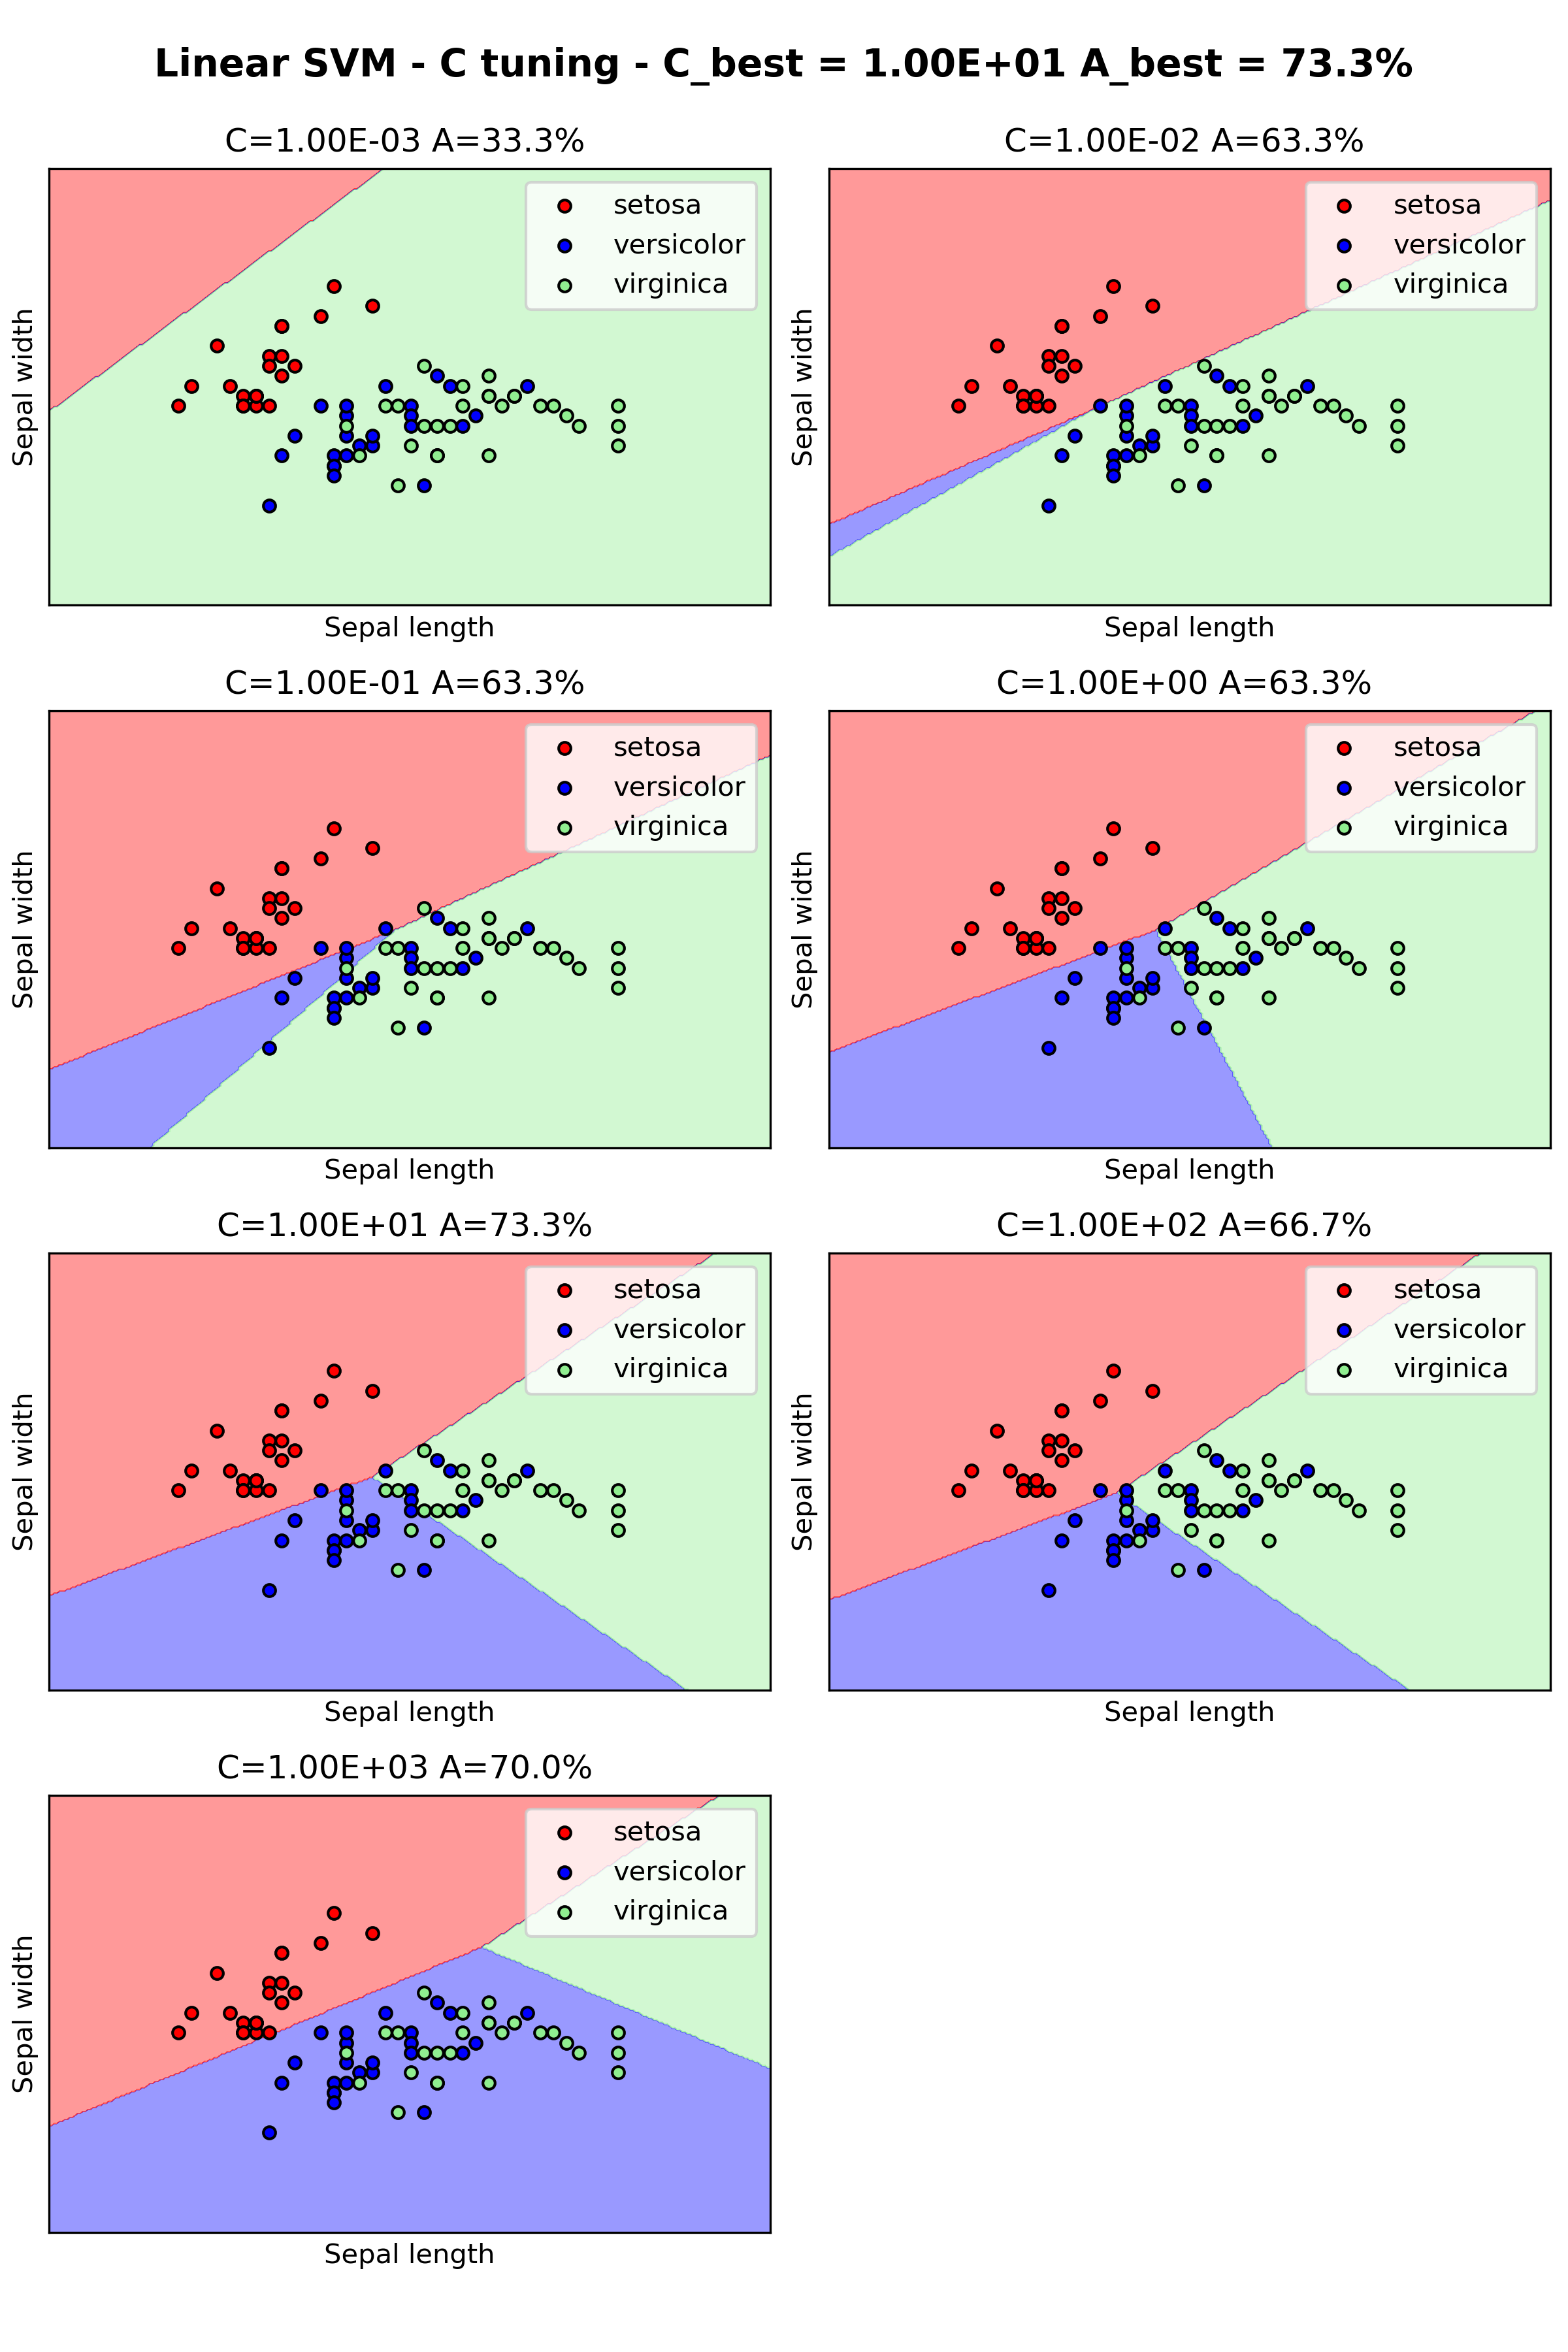
\includegraphics[height=0.8\paperheight]{img/fig01a.png}
		\caption{Decision Boundaries changing C in Linear SVM on Training set}
		\label{fig:linear1}
	\end{figure}

	\begin{figure}[ht!]
		\centering
		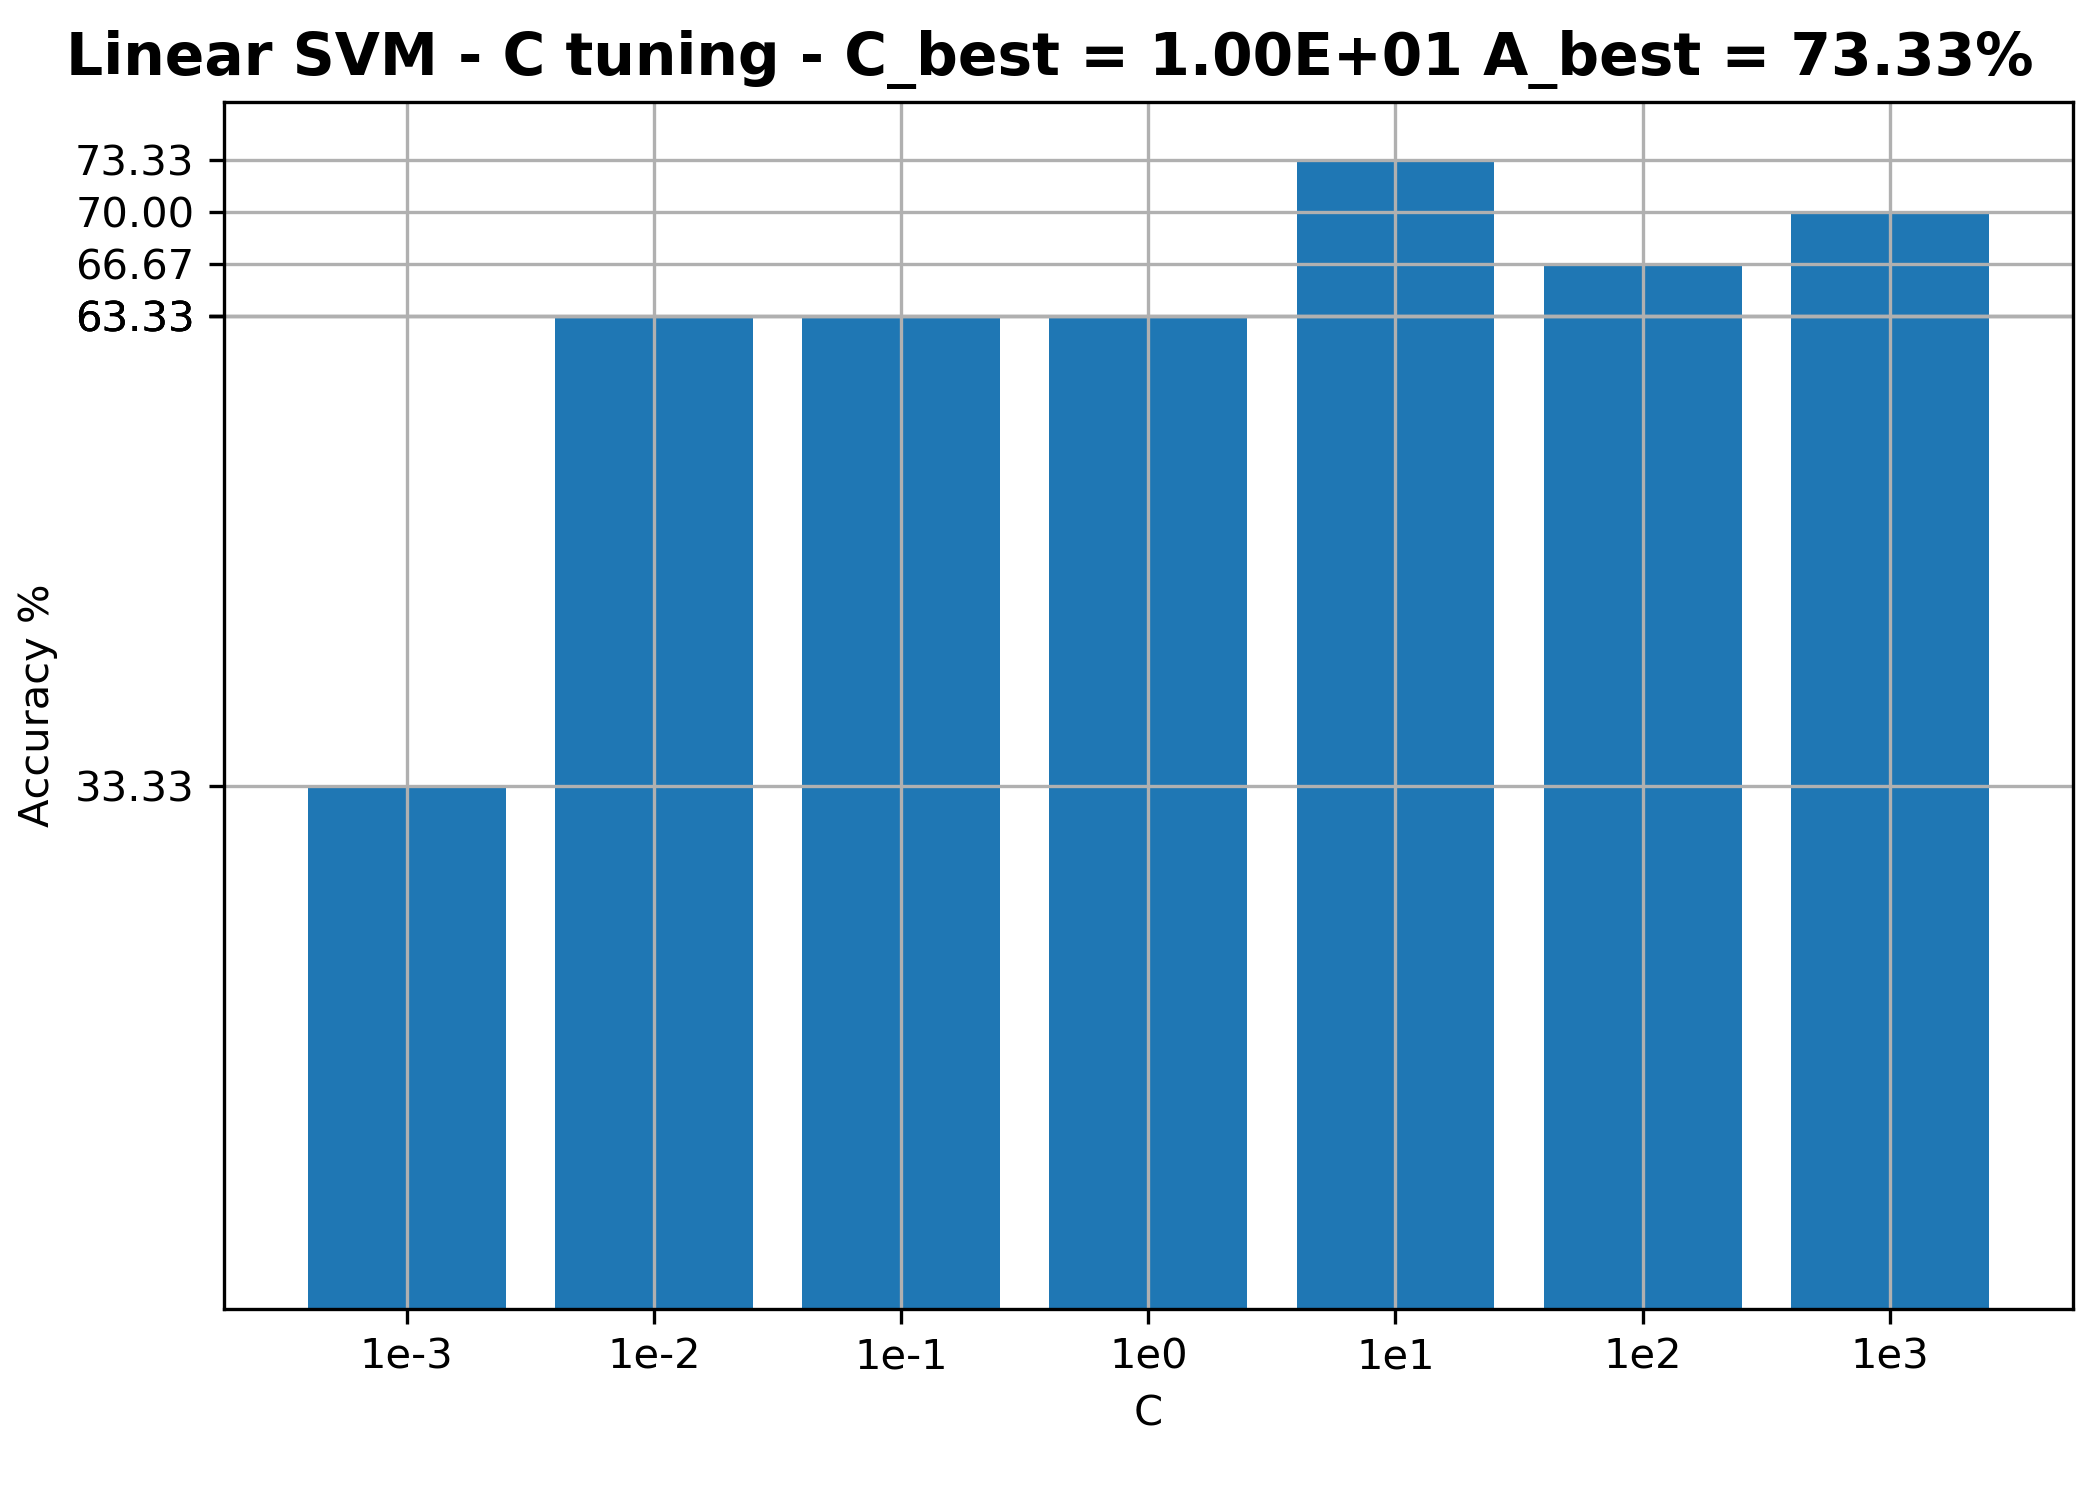
\includegraphics[width=0.7\paperwidth]{img/fig01b.png}
		\caption{Accuracy changing C in Linear SVM}
		\label{fig:linear2}
	\end{figure}

	\begin{figure}[ht!]
		\centering
		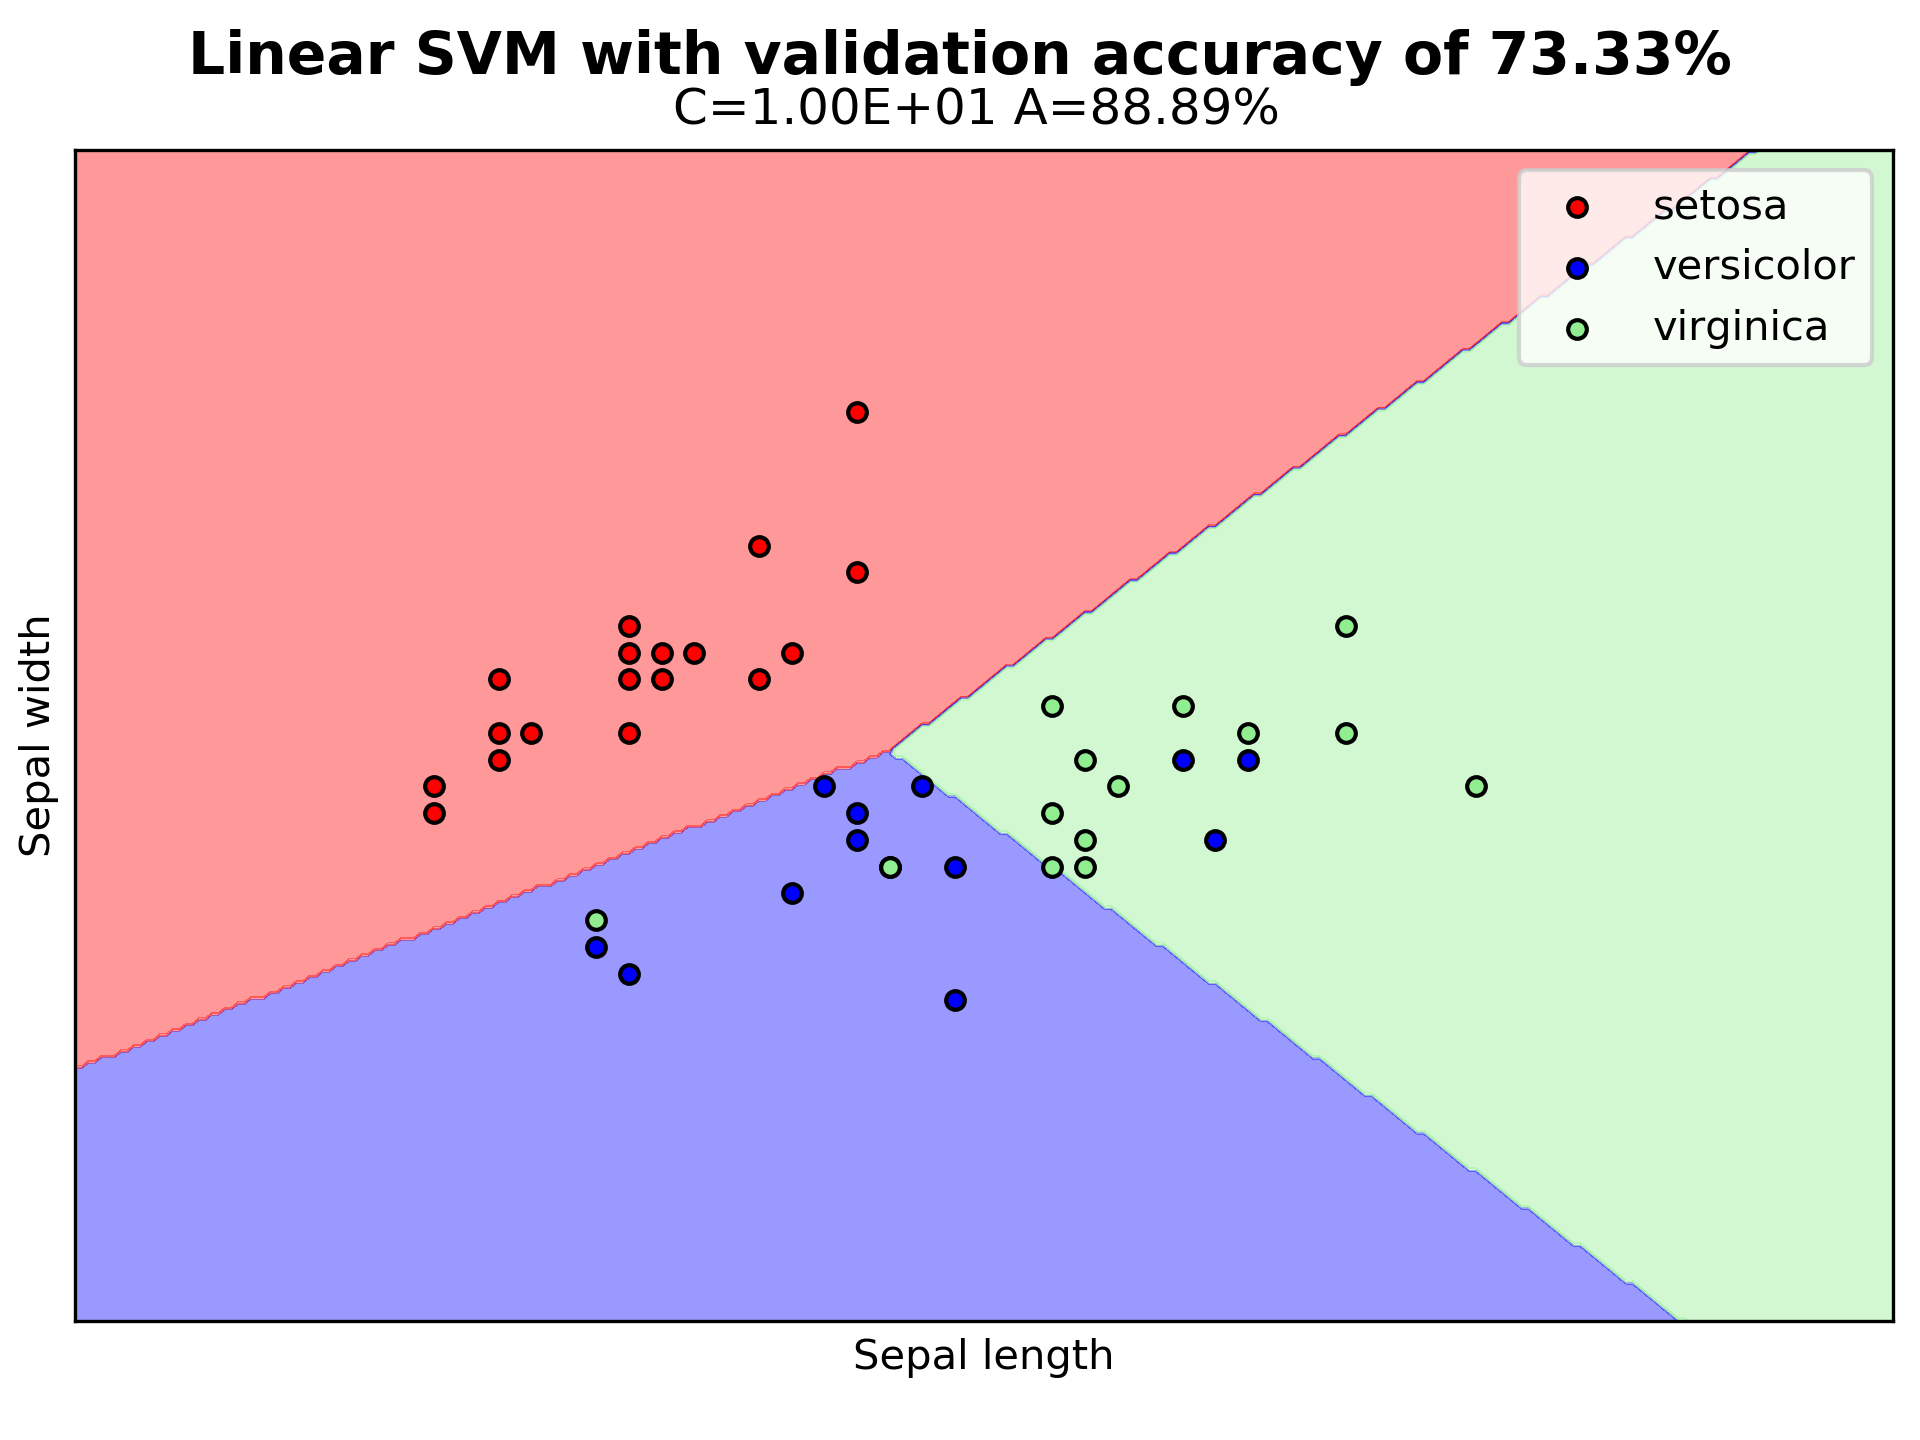
\includegraphics[width=0.7\paperwidth]{img/fig01c.png}
		\caption{Results on the test set}
		\label{fig:linear3}
	\end{figure}
		
	\section{RBF Kernel}
	
	In the second part of this homework I used SVM with RBF kernel. This time I had to find the best pair of $C$ and
	I standardized \texttt{x} using \texttt{StandardScaler} making each feature zero-mean and unit-variance. Then I applied PCA on the normalized X obtaining the projection using all $1087$ PCs as in \vref{lst:pca}.
	I decided to implement a custom function called \texttt{reconstruction()} in order to re-project \texttt{x\_t} using first $60$, $6$, $2$ and last $6$ principal component (PC) and visualize the reconstructed images with \texttt{show\_reconstruction()} function as you can see in \vref{lst:reconstruction}.
	
	
	
	\FloatBarrier
	
	\section{Classification}
		
	The formulation of Na\"ive Bayes is described in \cref{eq:1}.
	\begin{equation} \label{eq:1}
		\hat{y}=\argmax_{i \in \{1,\dots,k\}} p ( y_i \mid x_1, \dots, x_d) = \argmax_{i \in \{1,\dots,k\}}\overbrace{p(y_i)}^{Prior} \prod_{j=1}^{d}\overbrace{p(x_j\mid y_i)}^{Likelihood}
	\end{equation}
	where
	\begin{conditions}
		\hat{y_i}	&	predicted label \\
		y_i			&	$i$-th label with $i \in \{1,\dots,k\}$\\
		x_j			&  	$j$-th example with $j \in \{1,\dots,d\}$   \\   
		p(x\mid y) 	&	Gaussian
	\end{conditions}
	
	\section{Code Execution}
	\subsection{Requirements}
	\begin{itemize}
		\item Python 3
		\item All dependencies in \texttt{requirements.txt}.
		
		\texttt{\$ pip install -r requirements.txt} to install them
	\end{itemize}
	\subsection{Usage}
	\begin{itemize}
		\item \texttt{\$ python program.py -n <PACS\_homework folder>}
		
		Loads Image from the specified \texttt{<PACS\_homework folder>} and execute the code
		
		\item \texttt{\$ python program.py -s <PACS\_homework folder>}
		
		Loads Image from the specified \texttt{<PACS\_homework folder>} and save files in \texttt{data.npy} and \texttt{label.npy} for faster next execution before executing the code
		
		\item \texttt{\$ python main.py -l <data.npy file> <label.npy file> }
		
		Loads Image from \texttt{data.npy} and \texttt{label.npy} files and execute the code
	
	\end{itemize}
	\subsection{Reproducibility}
	In order to reproduce the same data for this experiment you have to change the global variable \texttt{r\_state} (line) from \texttt{None} to $252894$ which is my badge number.

	\section*{Attachments}
	%Make sure to change these
	\begin{itemize}
		\item Source Code:
		\begin{itemize}
			\item \texttt{main.py}
			\item \texttt{requirements.txt}
		\end{itemize}
	\end{itemize}
	%\fi %comment me out
	
	
	
%	\begin{thebibliography}{9}
%		\bibitem{Robotics} Fred G. Martin \emph{Robotics Explorations: A Hands-On Introduction to Engineering}. New Jersey: Prentice Hall.
%		\bibitem{Flueck}  Flueck, Alexander J. 2005. \emph{ECE 100}[online]. Chicago: Illinois Institute of Technology, Electrical and Computer Engineering Department, 2005 [cited 30
%		August 2005]. Available from World Wide Web: (http://www.ece.iit.edu/~flueck/ece100).
%	\end{thebibliography}
	
\end{document}
